\documentclass[11pt,twocolumn]{article}

\usepackage{times}
\usepackage{fullpage}

\usepackage{booktabs}  % for \midrule
%\usepackage{subfigure}
\usepackage{balance}
\usepackage{graphicx}
\usepackage{xspace}
%\usepackage{pslatex}
%\usepackage{pifont}
%\usepackage{multirow}
%\usepackage{array}
%\usepackage{booktabs}
%\usepackage{cite}
\usepackage{url}
%\usepackage{cancel}
\usepackage{color,colortbl}
%\usepackage{microtype}
%\usepackage{textcomp}% http://ctan.org/pkg/textcomp
\usepackage{tabularx}
\usepackage{framed}
\usepackage[]{algorithm2e}
\SetAlFnt{\small}
\SetAlCapFnt{\small}
\usepackage{algorithmic}

\usepackage{listings}
%\usepackage{scrextend}
%\usepackage{mathtools}
\usepackage{pbox}

\let\labelindent\relax
\usepackage{enumitem}

\usepackage{tikz}
\usetikzlibrary{arrows,automata}
\usetikzlibrary{calc,positioning}
\usepackage{lipsum,adjustbox}

%\usepackage{tikz}
%\usepackage{decorations.pathmorphing}
%\usepackage{assymb}

\usepackage[labelfont=bf]{caption}

%\theoremstyle{plain}
\newtheorem{theorem}{\bf{Theorem}}%[section]
\newtheorem{lemma}[theorem]{\bf{Lemma}}
\newtheorem{corollary}[theorem]{\bf{Corollary}}
\newtheorem{proofl}[theorem]{\bf{Proof}}
\newtheorem{proposition}[theorem]{\bf{Proposition}}

%\theoremstyle{definition}
\newtheorem{definition}{\bf{Definition}}%[section]
\newtheorem{observation}{\bf{Observation}}%[section] 

%\theoremstyle{remark}
\newtheorem{example}{\bf{Example}}
\newtheorem{notation}{\bf{Notation}}
\newtheorem{fact}{\bf{Fact}}

\usepackage{listings}
%%\usepackage{listings-golang}
\usepackage{color}

%\usepackage{sectsty}
%\sectionfont{\fontsize{12}{15}\selectfont}

\usepackage{hyperref}


\newcommand\mypara[1]{\vspace{.3em}\noindent\textbf{#1}}
\newcommand{\urlwofont}[1]{\urlstyle{same}\url{#1}}


%%%%%%%%%%%%%%%%%%%%%%%%%%%%%%%%%%%%%%%%
% Useful reviewing/feedback annotations
\usepackage{ifthen}
\usepackage[normalem]{ulem} % for \sout
\usepackage{xcolor}
\usepackage{amssymb}

\newcommand{\ra}{$\rightarrow$}
\newboolean{showedits}
\setboolean{showedits}{true} % toggle to show or hide edits
\ifthenelse{\boolean{showedits}}
{
	\newcommand{\ugh}[1]{\textcolor{red}{\uwave{#1}}} % please rephrase
	\newcommand{\ins}[1]{\textcolor{blue}{\uline{#1}}} % please insert
	\newcommand{\del}[1]{\textcolor{red}{\sout{#1}}} % please delete
	\newcommand{\chg}[2]{\textcolor{red}{\sout{#1}}{\ra}\textcolor{blue}{\uline{#2}}} % please change
}{
	\newcommand{\ugh}[1]{#1} % please rephrase
	\newcommand{\ins}[1]{#1} % please insert
	\newcommand{\del}[1]{} % please delete
	\newcommand{\chg}[2]{#2}
}

\newboolean{showcomments}
\setboolean{showcomments}{true}
%\setboolean{showcomments}{false}
\newcommand{\id}[1]{$-$Id: scgPaper.tex 32478 2010-04-29 09:11:32Z oscar $-$}
\newcommand{\yellowbox}[1]{\fcolorbox{gray}{yellow}{\bfseries\sffamily\scriptsize#1}}
\newcommand{\triangles}[1]{{\sf\small$\blacktriangleright$\textit{#1}$\blacktriangleleft$}}
\ifthenelse{\boolean{showcomments}}
%{\newcommand{\nb}[2]{{\yellowbox{#1}\triangles{#2}}}
{\newcommand{\nbc}[3]{
 {\colorbox{#3}{\bfseries\sffamily\scriptsize\textcolor{white}{#1}}}
 {\textcolor{#3}{\sf\small$\blacktriangleright$\textit{#2}$\blacktriangleleft$}}}
 \newcommand{\version}{\emph{\scriptsize\id}}}
{\newcommand{\nbc}[3]{}
 \renewcommand{\ugh}[1]{#1} % please rephrase
 \renewcommand{\ins}[1]{#1} % please insert
 \renewcommand{\del}[1]{} % please delete
 \renewcommand{\chg}[2]{#2} % please change
 \newcommand{\version}{}}
\newcommand{\nb}[2]{\nbc{#1}{#2}{orange}}

\definecolor{ibcolor}{rgb}{0.4,0.6,0.2}
\newcommand\iv[1]{\nbc{IB}{#1}{ibcolor}}
\usepackage{wasysym}
\newcommand\yesml[1]{\nbc{ML {\textcolor{yellow}\sun}}{#1}{mircolor}}

\definecolor{sgcolor}{rgb}{0.2,0.0,0.5}
\newcommand\sg[1]{\nbc{SG}{#1}{sgcolor}}

\definecolor{samcolor}{rgb}{0.2,0.4,0.2}
\newcommand\sam[1]{\nbc{SC}{#1}{samcolor}}

\definecolor{hccolor}{rgb}{0.21,0.54,0.84}
\newcommand\hc[1]{\nbc{HC}{#1}{hccolor}}

\definecolor{ideacolor}{rgb}{1.0,0,0.5}
\newcommand\idea[1]{\nbc{IDEA}{#1}{ideacolor}}


\definecolor{abstractcolor}{rgb}{0.0,0.5,1.0}
\newcommand\rabstract[1]{\nbc{ABSTRACT}{#1}{abstractcolor}}

\definecolor{introcolor}{rgb}{0.0,1.0,0.5}
\newcommand\rintro[1]{\nbc{INTRO}{#1}{introcolor}}

\definecolor{papercolor}{rgb}{1.0,1.0,0.0}
\newcommand\rpaper[1]{\nbc{PAPER}{#1}{papercolor}}

\definecolor{multicolor}{rgb}{1.0,0,0}
\newcommand\rmulti[1]{\nbc{MULTI}{#1}{multicolor}}

% Todo Command
\definecolor{todocolor}{rgb}{0.9,0.1,0.1}
\newcommand{\todo}[1]{\nbc{TODO}{#1}{todocolor}}


%%%%%%%%%%%%%%%%%%%%%%%%%%%%%%%%%%%%%%%%


\begin{document}

%\title{Inferring likely data invariants of distributed systems}
\title{Understanding the Network Performance of Graph Processing Frameworks}
\author{Anil Yelam, Audrey Randall}
\date{}

\maketitle

\begin{abstract}
\label{sec:abstract}
\small
\textit{In big data analytics, balanced execution of a computation is important for maximizing 
utilization of available resources in the cluster like CPU, Memory and Network. Various
works in the past have looked at optimized execution of big data platforms like Apache 
Hadoop MapReduce, Apache Spark and other sort and shuffle based workloads. In this paper,
we go on a similar quest for graph processing frameworks, which are equally commonly used
in big data processing and has not been hitherto well studied. We discuss various 
factors that affect the balanced execution of a graph processing algorithms on a given 
cluster. Specifically, we focus on the effect of different graph partitioning methods 
on performance of Pagerank algorithm on a wide range of natural graphs. By both studying 
the properties of these graphs and results from the pagerank runs on Apache Giraph, we show 
that even the simplest of the partitioning schemes can have a significant effect on the 
performance.}
\end{abstract}

\section{Introduction}
\label{sec:intro}
The importance of balanced execution of big data frameworks (Papers to link: 
Osterhout\cite{Ousterhout:2015:MSP:2789770.2789791}, Themis\cite{Rasmussen:2012:TIM:2391229.2391242}, 
TritonSort\cite{Rasmussen:2013:TBE:2427631.2427634}).

Why we picked graph processing.

What we did or found out, in a nutshell.


\section{Background}
\label{sec:background}

All about the graph processing frameworks and their computational models, basically 
a brief summary of \cite{Heidari:2018:SGP:3212709.3199523}. And a bunch of related 
papers we have read, like comparison papers \cite{Guo:2014:WGP:2650283.2650530,
Ammar:2018:EAD:3231751.3242935} and some earlier graph processing systems these papers 
point to - such as Pregel\cite{Malewicz:2010:PSL:1807167.1807184}, PowerGraph
\cite{Gonzalez:2012:PDG:2387880.2387883} and others.





\subsection{Apache Giraph}
\label{sec:giraph}

Apache Giraph\cite{ApacheGiraph} is a popular open-source implementation of
Pregel\cite{Malewicz:2010:PSL:1807167.1807184}. Giraph runs on Hadoop MapReduce and uses 
Map-only jobs to schedule and coordinate the 
vertex-centric workers and uses HDFS for storing and accessing graph datasets. 
It is developed in Java and has a large community of developers and users such as 
Facebook\cite{GiraphAtFacebook}. Giraph has a faster input loading time compared to Pregel 
because of using byte array for graph storage. On the other hand, this method 
is not efficient for graph mutations, which lead to decentralized edges when removing an edge. 
Giraph inherits the benefits and deficiencies of the Pregel vertex-centric
programming model. We picked Giraph for the supposed ease of use of this framework and the 
community support. 

We ran Giraph on a 4-node hadoop cluster. Each of these nodes are t2.xlarge AWS machines
each with 4 vCPUs, 16 GB Memory, 32 GB SSD and upto 1 Gbps Network. Giraph workers run 
as Map jobs, each in their YARN containers. YARN allows setting limits on the number of cores 
and memory to each container, so we limit each giraph worker to 1 vcore and 2 GB memory - so 
we could run a maximum of around 20 giraph workers given our cluster capacity. 
We chose PageRank as our graph algorithm since it is global and involves computation at all the vertices 
and  edges in every iteration. We ran five iterations of PageRank (called SuperSteps) on each 
graph, with the two partitioners that we implemented in Giraph  using \textit{HashPartitionerFactory} 
and \textit{SimpleLongRangePartitionerFactory} classes. The CPU usage on all the machines 
from a sample run of Giraph using round-robin partitioning on Facebook's Darwini graphs 
is shown in Figure \ref{fig:sample_giraph_run}.

\begin{figure}
	\centering
	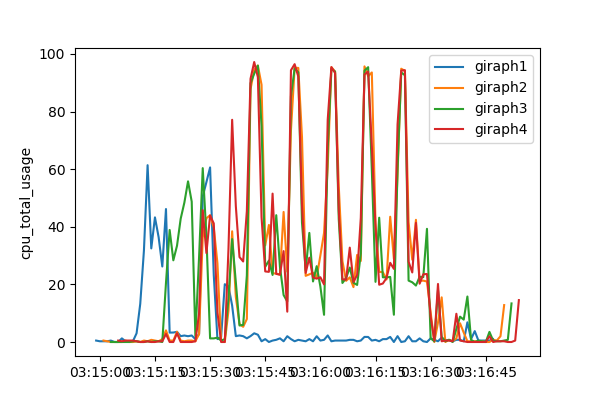
\includegraphics[width=\columnwidth]{./samplerun.png}
    \caption{CPU usage on all the nodes from a sample PageRank run over time. The five spikes 
        indicate five iterations of the algorithm.}
	\label{fig:sample_giraph_run}
\end{figure}

A significant amount of the time spent on this project was spent setting up our cluster and installing 
Giraph and all of its dependencies. Even for a well-supported and widely used piece of software like 
Giraph, this was a time consuming challenge. To begin with, version mismatches of Java, HDFS, Ubuntu, 
and Giraph itself caused a number of difficult-to-debug errors. For example, installing the most recent 
version of Java caused a mysterious build error that took hours to track down a workaround for (the workaround 
being to downgrade Java). Additionally, once Giraph had been successfully built, we spent eight 
hours tuning various settings before the example job provided in the documentation would run without error. 
This was due to a number of factors. First, configuration settings are scattered across many different files, 
making it challenging to identify the source of a problem and difficult to predict how the settings would interact 
with each other. Second, few facilities existed for fine-tuning resource allocation. Many jobs failed with 
``out of memory'' exceptions because it was difficult to tune the amount of memory they would be 
allocated. Third, error messages are not gathered in a central location - the existence of numerous log files made 
tracking down errors time consuming. Finally, Giraph seems to be a highly sensitive and delicate system. 
Unfortunately, as a result it is fragile: the slightest misallocation or imbalance of a resource causes jobs to 
fail with little explanation.

Given limited total memory capacity of our cluster (4*16 GB), we could only run medium sized graphs 
(with around 100 million edges) as Giraph does everything in memory. We ran PageRank on each of the graphs 
we discussed in previous section with both round-robin and range partitioners while varying the number of 
giraph workers (each with 2 GB memory) from 2 to 20. The execution times (excluding any preprocessing time) 
for these graphs using different partitioners are shown in Figures 
\ref{fig:giraph_roundrobin} and 
\ref{fig:giraph_range}. The missing data points for few input graphs at 2, 4 and 6 workers is due to the fact 
that these graphs are too big and cannot be run with fewer workers. 


\begin{figure}[!t]
	\centering
	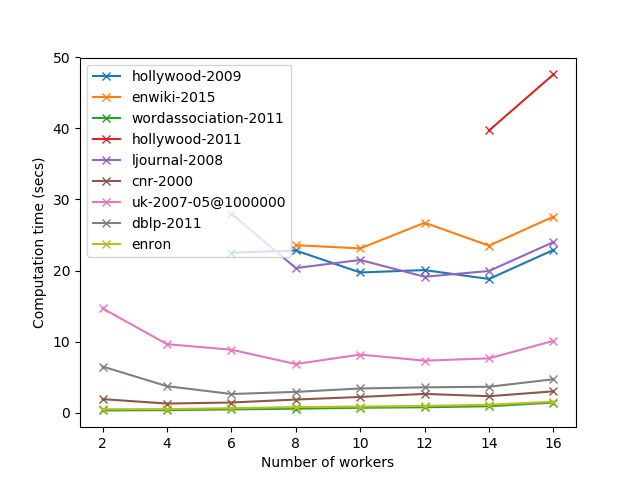
\includegraphics[width=\columnwidth]{./giraph_roundrobin.png}
    \caption{PageRank computation time for various graphs on Giraph with RoundRobin vertex partitioner
        as number of workers (partitions) are increased.}
	\label{fig:giraph_roundrobin}
\end{figure}

\begin{figure}[!t]
	\centering
	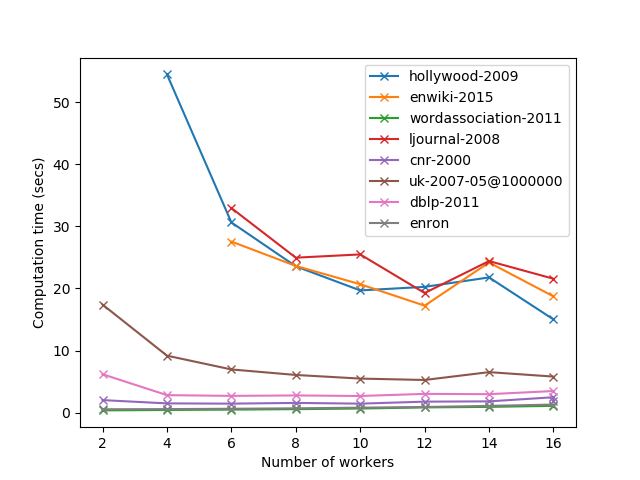
\includegraphics[width=\columnwidth]{./giraph_range.png}
    \caption{PageRank computation time for various graphs on Giraph with Range vertex partitioner
    as number of workers (partitions) are increased.}
	\label{fig:giraph_range}
\end{figure}

In both cases, we expected the computational time to go down as the number of workers increased, 
which only happened with the range partitioner. Computation times for range partitioner are less 
compared to round-robin partitioner for every graph, which seems to indicate that network overhead 
affects the performance more than straggler problems caused by the imbalance in partitioning.
In general, we didn't see the results we were expecting. Our conclusion was that Giraph has a 
lot of setup and preprocessing overheads that adds a lot of 
noise that significantly affects our runs since we use medium sized graphs that take only few seconds 
to run. We believe that 
using much larger graphs (like Twitter or Facebook) would give us the results that could let us 
clearly draw conclusions, but we could not run them due to resource limitations. We leave that to 
future work.

\section{Implementation}
\label{sec:impl}
Experimental setup and the steps involved, in detail.

%% Add other sections here


\balance
\vspace{-0.3cm}
{\footnotesize \bibliographystyle{acm}
\bibliography{paper}}
\vspace{-0.5cm}

\end{document}
